Separating dynamics, tracer and physics grids introduces the added complexity of having to map the state from dynamics and tracer grids to the physics grid; and mapping physics tracer tendencies back to the tracer grid and physics tendencies needed by the dynamical core to the dynamics grid. The dynamics grid refers to the Gauss-Lobatto-Legendre (GLL) quadrature nodes by the spectral-element method to solve the momentum equations for the momentum vector $(u,v)$, thermodynamics equation for temperature ($T$), continuity equation for dry air ($p$), and continuity equations for water vapor and condensates thermodynamically active \citep[see, e.g., ][ for details]{LetAl2018JAMES}. By tracer grid we refer to the $pg3$ grid on which CSLAM performs tracer transport of water vapor, condensates and other tracers. The GLL value for water vapor and condensates is overwritten by the CSLAM values every physics time-step so that the spectral-element advection of water species does not become decoupled from the the CSLAM advection of the same water species. Mapping velocity components, dry air mass and temperature from the GLL grid to the $pg2$ grid is done by using the internal degree 3 Lagrange basis functions in CAM-SE \citep[ as described in  ][ for pg3; exactly the same methods can be used for $pg2$]{HL2018MWR}.

As compared to the $pg3$ configuration, the extra complication of the $pg2$ setup is that tracer state needs to be mapped from the tracer grid to the physics grid and tracer tendencies need to the mapped from the physics grid to CSLAM grid. In order to describe the algorithm some notation needs to be introduced.

The mapping algorithm is applied to each element $\Omega$ (with spherical area $\Delta \Omega$) so without loss of generality consider one element. Let $\Delta A^{(pg)}_k$ and $\Delta A^{(nc)}_\ell$ be the spherical area of the physics grid grid cell $A^{(pg)}_k$ and CSLAM control volume $A^{(nc)}_\ell$, respectively. The physics grid cells and CSLAM cells respectively span the element without gaps or overlaps
\begin{eqnarray}
\cup_{k=1}^{pg^2}A^{(pg)}_k=\Omega \text{ and } A^{(pg)}_k \cap A^{(pg)}_\ell = \emptyset \quad \forall k\ne \ell,\\
\cup_{k=1}^{nc^2}A^{(nc)}_k=\Omega \text{ and } A^{(nc)}_k \cap A^{(nc)}_\ell = \emptyset \quad \forall k\ne \ell.
\end{eqnarray}
The overlap areas between the $k$-th physics grid cell and CSLAM cells is denoted
\begin{equation}
A_{k\ell}=A^{(pg)}_k \cap A^{(nc)}_\ell,
\end{equation}
so that
\begin{equation}
A^{(pg)}_k=\cup_{l=1}^{nc^2}A_{k\ell}.
\end{equation}
This overlap grid is also referred to as an exchange grid.
\subsection{Mapping tracers from CSLAM to $pg$}\label{sec:nctopg}
For mapping tracer state from the CSLAM grid to any physics grid can be done using exising CSLAM technology, i.e. do a high-order shape-preserving reconstruction of mixing ratio and dry air mass inside each CSLAM control volume and integrate those reconstruction functions over the overlap areas \citep{LNU2010JCP,NL2010JCP}. This algorithm retains the properties of CSLAM: inherent mass-conservation, mixing ratio shape-preservation and linear-correlation preservation. 

In mathematical terms, the dry pressure level thickness integrated over the $k$'th physics grid cell is given by
\begin{equation}
\overline{\Delta p}^{(pg)}_k=\sum_{\ell=1}^{nc^2}\langle \Delta p\rangle_{k\ell},
\end{equation}
where $\langle \Delta p\rangle_{k\ell}$ is the integral over the high-order reconstruction of $\Delta p$ over the overlap area $A_{k\ell}$ divided by the area of the overlap
\begin{equation}
\langle \Delta p\rangle_{k\ell}=\frac{1}{\delta A_{k\ell}}\int_{A_{k\ell}}\left[ \sum_{i+j\le 2}C^{(ij)}_\ell x^{i}y^{j}\right] dA,
\end{equation}
where the reconstruction coefficients $C^{(ij)}_\ell$ in CSLAM cell $\ell$ are computed from the cell average pressure level thicknesses on the CSLAM grid $\Delta p^{(nc)}$ and the numerical integration over overlap areas is done by line-integral quadrature. The details are given in \cite{LNU2010JCP} and not repeated here.

The tracer mass per unit area on the physics grid is given by
\begin{equation}
\overline{m\Delta p}^{(pg)}_k=\sum_{\ell=1}^{nc^2}\langle m\Delta p\rangle_{k\ell},
\end{equation}
where $\langle m\Delta p\rangle_{k\ell}$ is the integral over the high-order reconstruction of $\Delta p$ and $m$ combined using the approach outlined in Appendix B of \cite{NL2010JCP} over the overlap area $A_{k\ell}$
\begin{equation}
\langle m\Delta p\rangle_{k\ell}=\frac{1}{\delta A_{k\ell}}\int_{A_{k\ell}}\left[ \overline{\Delta p}_\ell^{(nc)}\sum_{i+j\le 2}c^{(ij)}_\ell x^{i}y^{j}+{\overline{m}}_\ell^{(nc)}\sum_{i+j\le 2}{\tilde{C}}^{(ij)}_\ell x^{i}y^{j}\right] dA,
\end{equation}
where ${\tilde{C}}^{(00)}_\ell=C^{(00)}_\ell-\overline{\Delta p}^{(nc)}_\ell$ and ${\tilde{C}}^{(ij)}_\ell=C^{(ij)}_\ell$ for $i,j>0$. The mixing ratio on the physics grid is then
\begin{equation}
\overline{m}^{(pg)}_k=\frac{\overline{m\Delta p}^{(pg)}_k}{\overline{\Delta p}^{(pg)}_k}.
\end{equation}



The tendencies from the parameterizations are computed on the physics grid. The tracer tendency in physics grid cell $k$ is denoted $f_k^{(pg)}$. The problem is how to map $f_k^{(pg)}$ to the CSLAM control volumes $f^{(nc)}$ satisfying the following constraints:
\begin{enumerate}
\item {\bf{Local mass-conservation}}
\begin{equation}
f_k^{(pg)}\Delta p^{(pg)}_k=\cup_{\ell=1}^{nc^2}\Delta A_{k\ell}\Delta p^{(nc)}_\ell f^{(nc)}_\ell,
\end{equation}
where $\Delta p^{(pg)}_k$ is the pressure level thickness in physics grid cell $k$ and similarly for $\Delta p^{(nc)}$.
\item {\bf{Shape-preservation in mixing ratio}}: The tendencies mapped to the CSLAM grid should not produce values smaller than the updated physics grid mixing ratios, $m^{(pg)}_k+\Delta tf_k^{(pg)}$, or values smaller than the existing CSLAM mixing ratios [revise for whatever code works best]
\begin{equation}
m^{(min)}=\min \left( m^{(pg)}_k+\Delta t f_k^{(pg)},\left\{ m^{(nc)}_{\ell} |\ell=1,nc^2\right\} \right),
\end{equation}
where $\Delta t$ is the physics time-step. Similarly for maxima
\begin{equation}
m_k^{(max)}=\max \left( m^{(pg)}_k+\Delta t f_k^{(pg)},\left\{ m^{(nc)}_{k\ell} |\ell=1,nc^2\right\} \right),
\end{equation}
\item {\bf{Linear correlation preservation}}: The physics forcing must not disrupt linear tracer correlation between species on the CSLAM grid \citep[see, e.g., ][]{LT2011QJR}.
\item {\bf{Consistency}}: A constant mixing ratio tendency, $cnst$, on the physics grid, $f_k^{(pg)}=cnst$ $\forall k$, must result in the same (constant) forcing on the CSLAM grid, $f_\ell^{(nc)}=f_k^{(pg)}=cnst$ $\forall \ell$.
\end{enumerate}
To motivate the algorithm that will simultaneously satisfy 1-4 it is informative to discuss how `standard' mapping algorithms will violate one or more of the constraints:
\begin{itemize}
\item Conservative remapping: Assume that one remaps the mass-tendencies in exactly the same way as the mapping of mixing ratio state from the CSLAM grid to the physics grid described in section \ref{sec:nctopg}. That is, replace $m$ with $f$ and map from physics grid to the CSLAM grid instead of the other way around. The mapped mass-tendency is $\overline{f\Delta p}^{(pg)}_k$ and due to the properties of the mapping algorithm the mass-tendency is conserved, linear correlation between mass-tendencies are conserved and shape in mass-tendency is preserved.

That said, this approach is problematic. The issue is that the dry pressure level thickness mapped from $pg$ to $nc$, call it $\widetilde{\overline{\Delta p}}^{(nc)}$, differs from $\overline{\Delta p}^{(nc)}$. During physics-dynamics coupling the dry pressure level thickness should remain constant. So when converting the mass-tendencies to mixing ratio tendencies through, e.g.,
\begin{equation}
\overline{m}^{(pg)}_k=\frac{\overline{f\Delta p}^{(pg)}_k}{\overline{\Delta p}^{(pg)}_k},
\end{equation}
a constant mixing ratio tendency is not conserved since $\widetilde{\overline{\Delta p}}^{(pg)}_k\ne {\overline{\Delta p}}^{(pg)}_k$. Basically the constant tendency will map to a field representing the spurious discrepancy between $\widetilde{\overline{\Delta p}}^{(pg)}_k$ and ${\overline{\Delta p}}^{(pg)}_k$. A constant tendency can be preserved by using
\begin{equation}
\overline{m}^{(pg)}_k=\frac{\overline{f\Delta p}^{(pg)}_k}{\widetilde{\overline{\Delta p}}^{(pg)}_k},
\end{equation}
instead, but now mass-conservation is lost since $\widetilde{\overline{\Delta p}}^{(pg)}_k\ne {\overline{\Delta p}}^{(pg)}_k$. This issue is similar to the mass-wind inconsistency found in specified dynamics applications \citep[e.g.][]{JKLSBCRE2001QJR}. 

\begin{figure}[t]
\begin{center}
\noindent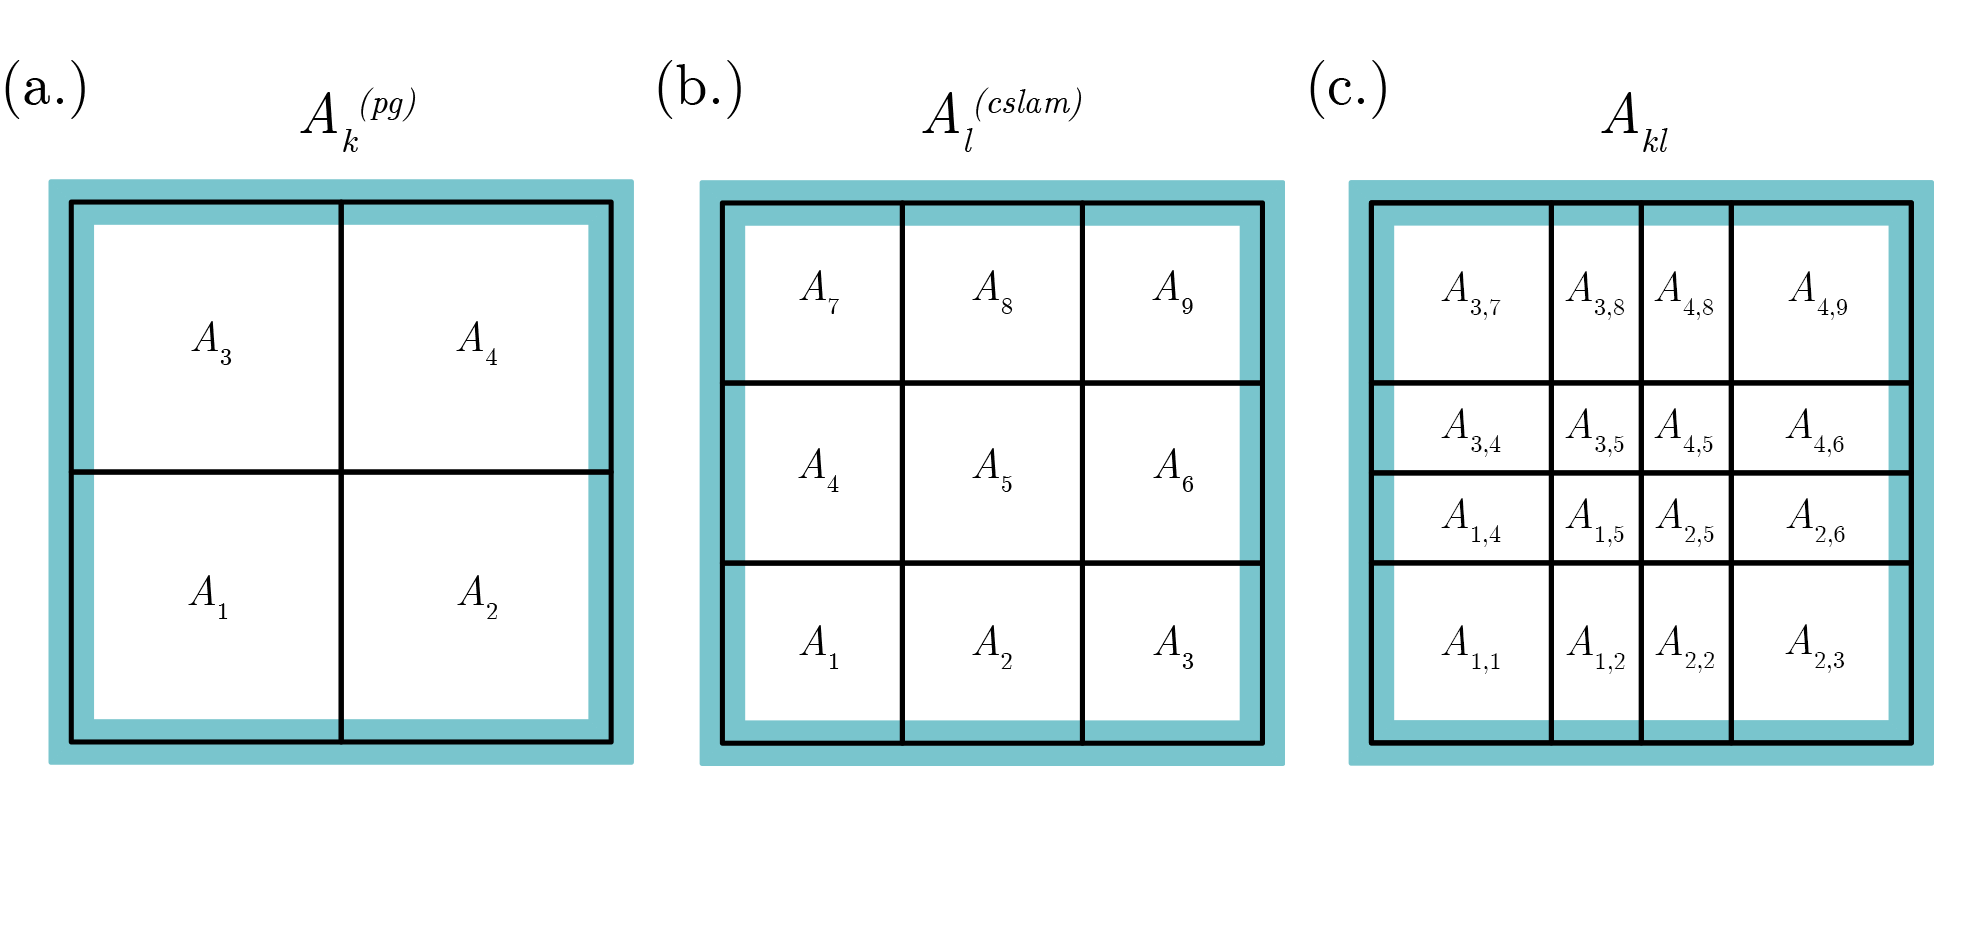
\includegraphics[width=30pc,angle=0]{figs/area-schematic.png}\\
\end{center}
\caption{Indice notation for (a) the $pg2$ grid, (b) the $pg3$ grid and (c) their exchange grid. {\color{red}Peter - do you think you will use this figure?}}
\label{fig:area-schematic}
\end{figure}

\begin{figure}[t]
\begin{center}
\noindent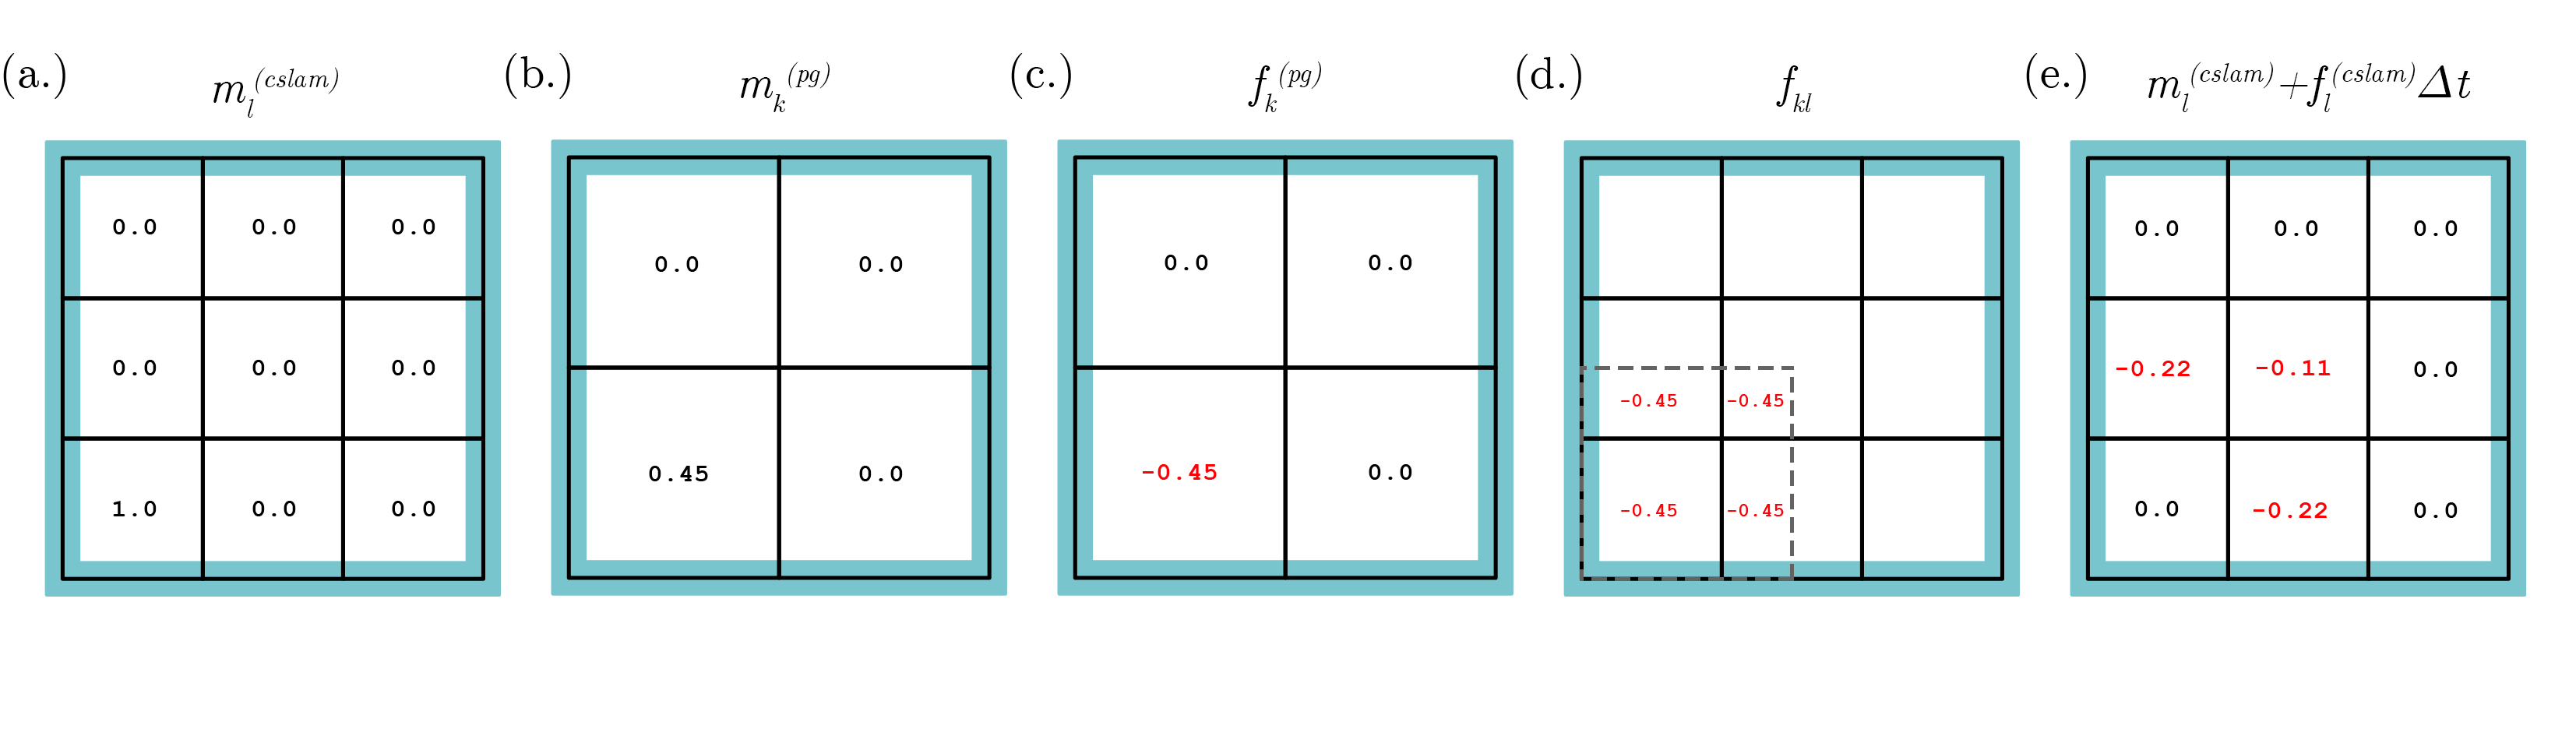
\includegraphics[width=30pc,angle=0]{figs/alg-schematic.png}\\
\end{center}
\caption{Make captions stand-alone while being concise}
\label{fig:alg-schematic}
\end{figure}

Even if one could derive a reversible map for mapping $\Delta p$ from physics grid to the CSLAM grid there could still be problems with driving mixing ratios negative on the CSLAM grid (we refer to this as the `negativity problem'). This problem is depicted schematically in Figure~\ref{fig:alg-schematic}. Consider a single element of CSLAM control volumes, containing only a single cell with mixing ratio $1.0$, and $0.0$ everywhere else ($m_l$; Figure ~\ref{fig:alg-schematic}a). Assume that the mixing ratios mapped to the $pg2$ grid ($m_k$; Figure~\ref{fig:alg-schematic}b) results in a negative tracer tendency from the physics ($f_k$; Figure~\ref{fig:alg-schematic}c). The non-zero values of the tendencies for $pg2$ areas overlapping CSLAM grid cells originally containing a mixing ratio of zero ($f_{k,l}$; Figure~\ref{fig:alg-schematic}d), are driven negative by the mapped tendency (Figure~\ref{fig:alg-schematic}e). 

%In the $pg2$ configuration, mapping the fields to and from the quadrature grid and $pg2$ grid is identical to that described in H18. As discussed above above, in mapping to the physics grid, CAM-SE's Lagrange basis functions are integrated over the $pg2$ control volumes to provide the physics with a volume averaged state. The procedure is accurate to machine precision, conserves thermal energy and dry air mass, and is consistent (i.e., the mapping preserves a constant). The reverse mapping, from the physics grid to the quadrature grid, is done using a tensor-product Lagrange interpolation (see Appendix A in H18). The Lagrange interpolation is consistent, conserves dry air mass ({\color{red}{Peter, is this true?}}), but does not conserve thermal energy. Errors arising from the lack of energy conservation were estimated to be small; about two orders of magnitude less than the energy dissipation due to the dynamical core alone.

%The semi-Lagrangian advection of tracers in our $pg2$ configuration is solved on the CSLAM grid. 





\item Interpolation: Traditional Lagrange interpolate of the mixing ratio tendency would preserve a constant and could be made shape-preserving using {\em{ad hoc}} filters \citep[e.g.][]{BC2002MWR} but will not inherently preserve mass tendency and suffers from the `negativity problem' described above.
\end{itemize}
As illustrated above none of the standard interpolation or remapping methods will simultaneously satisfy 1-4.
\subsection{Algorithm}
{\color{red}{mention that the reason we map tendency and not state is to avoid spurious tendencies solely due to interpolation errors, i.e. zero tendency on physics grid would transform into tendencies on the CSLAM grid.}}
Define the $\Delta m_{k\ell}$ is the amount of mixing ratio that can be removed without producing new extrema in $m_{k\ell}$
\begin{equation}
\Delta m_{k\ell}=\overline{m}_{k\ell}-m^{(min)},
\end{equation}
where $\overline{m}_{k\ell}$ has been computed using higher-order mapping ....
{\color{red}{mention why the problem is well-posed}}
